\section{Motivations}
\label{sec:motivation}

We focus on computation-heavy ML applications that are beyond the capabilities
of end devices. In this chapter, we will first show the heterogeneity of swarm
platforms for heavy computation and demonstrate that simple offloading does not
provide consistent response times in the presence of network and workload
variation. We then motivate computation adaptation by showing the trade-off
between application accuracy and processing times in two cases: different
algorithms and different parameters. At last, we summarize the challenges
associated with building an accurate performance model.

\subsection{Heterogeneous Environment}

\begin{figure}
  \begin{minipage}{0.4\textwidth}
    \centering
    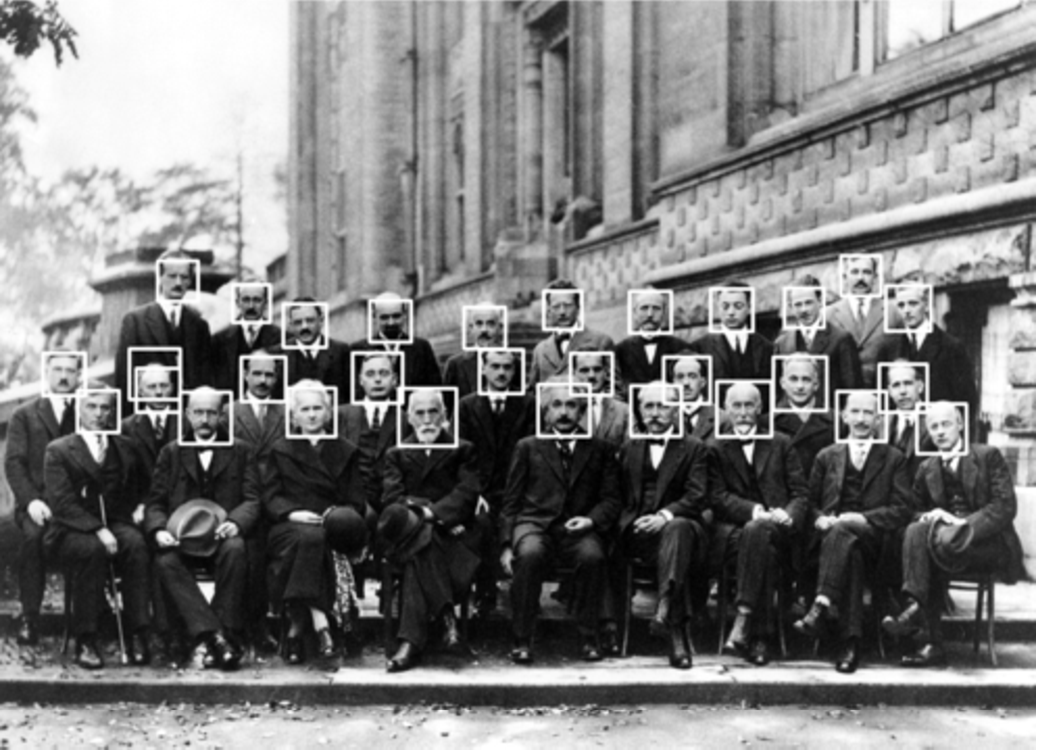
\includegraphics[width=.9\textwidth]{figures/physicist.pdf}
    \label{fig:physicist}
  \end{minipage}%
  \begin{minipage}{0.6\textwidth}
    \centering
    \begin{tabular}{c c c}
      \toprule
      \specialcell{RPi\\Model B}
      & \specialcell{Macbook \\ Model A1502}
      & \specialcell{Workstation\\Xeon E5-1620} \\
      \midrule
      4105 ms & 544 ms & 346 ms \\
      \bottomrule
    \end{tabular}
  \end{minipage}
  \caption{(Left) Face detection with a photograph of the Fifth Solvay
    International Conference on Electrons and Photons. (Right) Processing times
    using Viola-Jones face detector on different machines,with default OpenCV
    parameters.}
  \label{fig:capabilities}
\end{figure}

Our target application environment consists of machines with large range of
computing resources. Earlier, \autoref{sec:swarm-platforms} and
\autoref{tab:embedded} have discussed this dizzying array of machines ranging
from powerful computing units to low-power microcontrollers.  Low-power devices,
such as mobile phones or IoT microcontrollers, are significantly limited in
their processing capabilities. Performing ML inference easily takes seconds to
complete. As shown in \autoref{fig:capabilities}, to detect faces in a photo of
the Fifth Solvay International Conference on Electrons and Photons,\footnote{The
  original image (3000$\times$2171 pixels) is from Wikimedia and in the public
  domain.} it takes more than 4 seconds on a Raspberry Pi (Model B).

One technique is to use the edge and/or the cloud for offloading. While they are
substantially more powerful (7.5$\times$ to 11.9$\times$ in the face detection
task), both the edge and the cloud suffer from variable latency, unstable
connection, and service contention. These issues make it difficult to provide
consistent response times, especially for tail performance. \autoref{fig:edge}
shows the characteristics of end devices, the edge, and the cloud. We then
empirically validate the network variation and workload variation
(\autoref{fig:variation}).

\para{Network Variation.} We use the raw data in January 2016 from FCC
\href{https://www.fcc.gov/general/measuring-broadband-america}{Measuring
  Broadband America Program}~\cite{fcc} to validate the large variation in wide
area network. \autoref{fig:fcc-latency} shows the empirical cumulative
distribution function (ECDF) of measured network latency. \textit{Ping} time refers to
the round trip time (RTT) of ICMP echo requests from measurement devices to a
set of target test nodes. \textit{Download} and \textit{Upload} are latency
measured when performing downstream or upstream speed tests. From this figure,
we can see that the latency has 2-3 orders of magnitude difference. The
situation is worse with active traffic. The median network delay increases from
\SI{22}{\ms} to \SI{80}{\ms} under downstream load and \SI{272}{\ms} under
upstream load.

\para{Workload Variation.} \noindent We measure end-to-end latency with
TensorFlow serving~\cite{olston2017tensorflow}, a state-of-the-art serving
system for machine learning models. Specifically, we use
MNIST~\cite{lecun1998mnist} as a case study and study the serving performance
with different level of background load. \autoref{fig:tf-latency} shows the ECDF
with no load, 1K requests per second (RPS) and 5K RPS. From this figure, we can
see that the serving latency has significantly increased when the load
increases. With 1k load, 99.9 percentile latency increases from \SI{3.5}{\ms} to
\SI{22.5}{\ms}. With 5K load, even the median latency increases to
\SI{21.5}{\ms}: a 22.4$\times$ increase from \SI{0.96}{\ms} with no load.

\begin{figure}
  \centering
  \begin{subfigure}[t]{0.4\columnwidth}
    \centering
    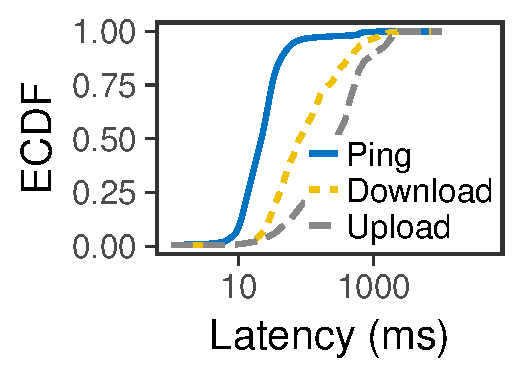
\includegraphics[width=\textwidth]{figures/fcc_latency.pdf}
    \caption{Broadband network latency.}
    \label{fig:fcc-latency}
  \end{subfigure}
  \hspace{2em}
  \begin{subfigure}[t]{0.4\columnwidth}
    \centering
    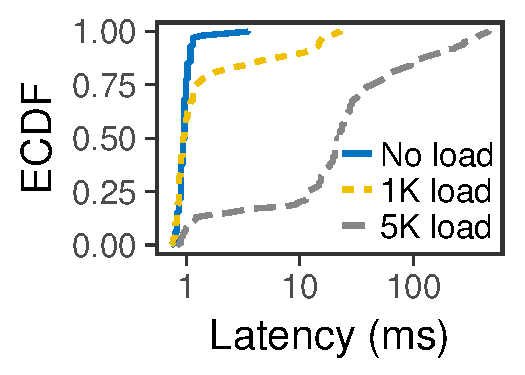
\includegraphics[width=\textwidth]{figures/tf_latency.pdf}
    \caption{TensorFlow serving latency.}
    \label{fig:tf-latency}
  \end{subfigure}
  \caption{(Left) WAN network latency has variation and the latency deteriorates
    during downstream and upstream speed tests. (Right) Server processing
    latency has variation and the latency deteriorates during load increase.}
  \label{fig:variation}
\end{figure}

\subsection{Accuracy-Time Tradeoff}
\label{sec:comp-perf-model}

\begin{figure}[t]
  \centering
  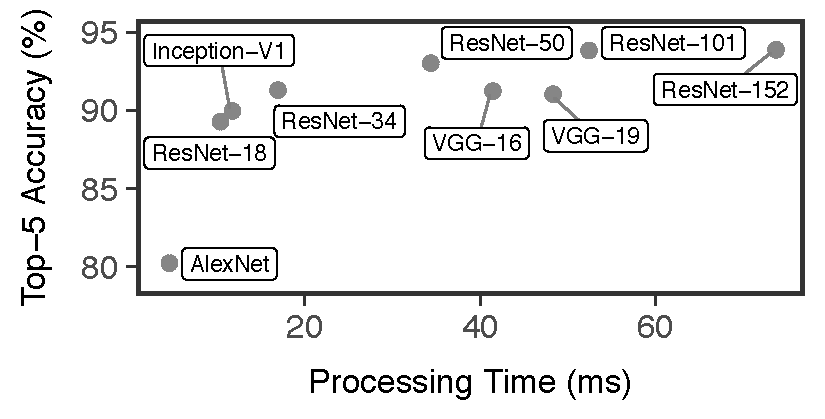
\includegraphics[width=.7\columnwidth]{figures/tradeoff-cnn.pdf}
  \caption{Benchmarks for popular CNN models demonstrate the trade-off between
    application accuracy and processing times. For data source and details,
    refer to
    \href{https://github.com/jcjohnson/cnn-benchmarks}{cnn-benchmarks}~\cite{cnn.benchmarks}.
  }
  \label{fig:cnn-tradeoff}
\end{figure}

Many tasks, especially ML inference, have multiple algorithms, or tunable
parameters for the same algorithm. These options result in different application
accuracy and processing times. As a result, we can speed up a computation task
by sacrificing accuracy. In this way, many tasks become tractable on end
devices. Servers can also tune their computation to accommodate network delays
or address heavy load. Below we show two examples.

\para{Convolutional Neural Networks (CNN)}. For the past few years, deep
learning and neural networks have gained attention in performing complex machine
learning tasks~\cite{goodfellow2016deep}. Convolutional neural networks (CNNs)
are particularly powerful for computer vision tasks, such as object detection
and image classification. There are many networks available:
AlexNet~\cite{krizhevsky2012imagenet}, Inception~\cite{szegedy2015going},
VGG~\cite{simonyan2014very}, ResNet~\cite{he2016deep}, etc. Huang et al. have
observed the speed/accuracy trade-off and explored this trade-off in an
exhaustive and fair manner~\cite{huang2016speed}. Because this thesis is not an
extensive study of neural networks, we only summarize one benchmark result in
\autoref{fig:cnn-tradeoff}. The processing times vary from \SI{4.3}{\ms} to
\SI{73.5}{\ms} and the accuracy\footnote{Top-5 accuracy here means that the
  correct label is one of the top five predictions made by the network.} varies
from 80.2\% to 93.8\%.

\para{Viola-Jones Face Detector.} This is an example of how tunable parameters
affect processing times and application accuracy. Viola-Jones (VJ) face
detector~\cite{viola2001rapid} detects face by moving a window over the image.
To detect faces at different sizes, it runs over an image pyramid with a
configurable scale. After the detection, there are typically multiple
neighboring windows with high scores close to the correct location of objects.
A post-processing step uses non-maximum suppression (NMS) to group detection
into a single bounding box. OpenCV~\cite{opencvlibrary} provides
\texttt{CascadeClassifier} with the following parameters,

\begin{itemize}[noitemsep, topsep=0pt]
\item \texttt{min\_size}: minimum detectable object size.
\item \texttt{scale}: how much image size is reduced at each image scale.
\item \texttt{min\_neighbors}: how many neighbors each candidate rectangle should
  have to retain it.
\end{itemize}

\begin{figure}[t]
  \centering
  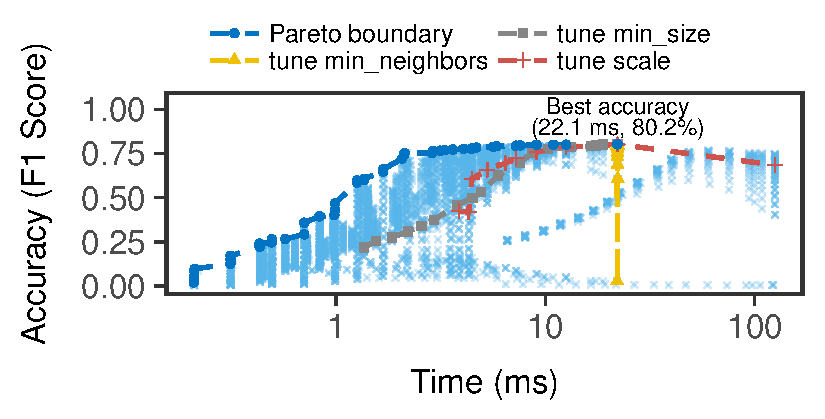
\includegraphics[width=.8\columnwidth]{figures/exhaustive-face.pdf}
  \caption{Benchmarks for Viola-Jones face detector with different
    parameters. These parameters form a large space that make performance
    modeling challenging.}
  \label{fig:vj-tradeoff}
\end{figure}

\autoref{fig:vj-tradeoff} shows how these parameters affect processing times and
accuracy. We measured the performance of 4,000 different parameter
configurations\footnote{\texttt{min\_size} ranges from 0 to 190, with a step
  size of 10; \texttt{scale} ranges from 1.01 to 1.46, with a step size of 0.05;
  \texttt{min\_neighbors} ranges from 0 to 19, with a step size of 1.} using
FDDB dataset~\cite{jain2010fddb}. In the figure, each cross dot represents the
processing time and application accuracy for one configuration. As we can see,
there is a tradeoff space: the processing times vary across almost 3 orders of
magnitude; the accuracy can be as low as 0\% and as high as 80.2\%.

% scale factor: 1.01..0.05..1.46 (10)
% min neighbors: 0..1..19
% min size: 0..10..190

\subsection{Performance Modeling and Challenges}
\label{sec:perf-model-chall}

We need to build the performance model to exploit the tradeoff between accuracy
and processing times. Because each algorithm is fundamentally different from
another one, we must exhaustively evaluate all available algorithms. For the
same algorithm with different parameters, exhaustive search can be prohibitively
expensive as the parameters form a combinatorial
space. \autoref{fig:vj-tradeoff} shows an evaluation of 4,000 parameter
configurations for Viola-Jones, which only has three parameters. A more complex
algorithm can have a staggering number of tunable parameters. For example,
HOG~\cite{dalal2005histograms} in OpenCV has the following parameters:
\texttt{win\_size}, \texttt{win\_stride}, \texttt{block\_size},
\texttt{block\_stride}, \texttt{cell\_size}, \texttt{nbins},
\texttt{win\_sigma}, \texttt{nlevels}, \texttt{hit\_threshold},
\texttt{padding}, \texttt{group\_threshold}, \texttt{use\_meanshift\_grouping},
etc.

A comprehensive performance modeling is actually not necessary. Instead, we only
need configurations that provide the best accuracy for a given processing time
constrain, i.e., the Pareto-optimal points. \autoref{fig:vj-tradeoff} highlights
the Pareto boundary in blue. We defer a formal definition of the Pareto-optimal
set in \autoref{sec:problem-formulation}.

In practice, we can reduce the number of samples further. The Pareto-optimal set
only needs to be accurate enough to distinguish near-optimal configurations from
the rest. Previous work has used two solutions: $(i)$ \textit{Random search.}
This simple approach samples the parameter space randomly and search/profile
with a budget. It is obvious that as the budget increases, the coverage improves
and the Pareto-optimal set is closer to the correct set. $(ii)$
\textit{Coordinate search.} This greedy approach starts with a random
configuration, moves along one parameter dimension if it improves, and stops
when it reaches a local optimum. After reaching the local optimum, if we still
have search budget, this approach repeats by picking another random
configuration.

Both random search and coordinate search have their problems. Random search
needs a lot of samples to approximate the real Pareto boundary. Coordinate
search may stuck in some local region and exhaust the search budget. As a
result, with a limit budget, both approaches could return sub-optimal points in
the trade-off space.

In addition, our discussion on performance modeling by far has not taken into
account of the heterogeneous capabilities of devices. What we have shown in
\autoref{fig:vj-tradeoff} is measured on a workstation with Xeon E5-1620 CPU;
the performance model will be different on another device, e.g., a Raspberry Pi.

%%% Local Variables:
%%% mode: latex
%%% TeX-master: "../compute"
%%% End:
